% 3. The relevant data exploration process (pre-processing, feature extraction/selection,
% clustering and visualization)


\section{Data exploration process}

\subsection{Pre-processing}
\subsubsection{Treatment of missing values}
Our dataset do not have missing values, so there is no need to treat them.
\subsubsection{Treatment of anomalous values}
\red{Quizá hay que quitar algunas personas por ser demasiado jóvenes comparadas con el resto}

The age of the patients is not well distributed. Most of them are over 60 years old, and only 4 of the patients are under 40. Due to this, it is very likely that the conclusions of our study will only be applicable to the elder people. However, we are reluctant to remove the younger patients.

\subsubsection{Treatment of incoherent values}
The variable FEV1 which is the Forced Expiratory Volume in 1 second, shows a few anomalously high values. Depending on factors like age and sex of a patient the average value of the FEV1 \red{should be} is around 3-6 litres, whereas the dataset shows values up to 86. As most of the values are within 0 and 10 we assume that the dataset contains the FEV1 in litres. To decide which values are to be determined as outliers we calculate the FEV1/FVC ratio which gives the percentage of the lung volume exhaled in the first second over the whole exhaled volume. All patients having a unrealistic ratio higher than 100\%, which are 22 patients, are determined to be outliers and eliminated. We chose not to apply any stricter constraints because the dataset does not include the sex of the patients which influences the normal values of the FEV1 much.

Source of knowledge about FEV1 and FVC:
https://www.nuvoair.com/blogs/blog/do-you-know-how-to-interpret-the-results-of-your-spirometry-test

\red{El enlace antiguo ha caido, ahora es este:}

\red{https://www.nuvoair.com/do-you-know-how-to-interpret-the-results-of-your-spirometry-test.html}

% \red{No sé si por outliers se entiende a datos que son verdad pero que son
% raros o si son datos que no son correctos, porque se van demasiado}

\red{Referenciar quizá el histograma con FEV1}
\red{Poner bien la referencia a la página}


% \todo[inline]{Redactar que FEV1 está mal, referenciar algún artículo que hable
% sobre el tema y para justificar que está mal, decidir qué haremos con esos pacientes (eliminarlos, o inferir
% sus valores de FEV1 en función de sus vecinos) y si los inferimos poner el proceso
% como lo hemos hecho}
% \red{El FEV1 tiene valores incoherentes. La mayoría están sobre 3, pero algunos
% están sobre 60}
\begin{figure}[bh]
\centering
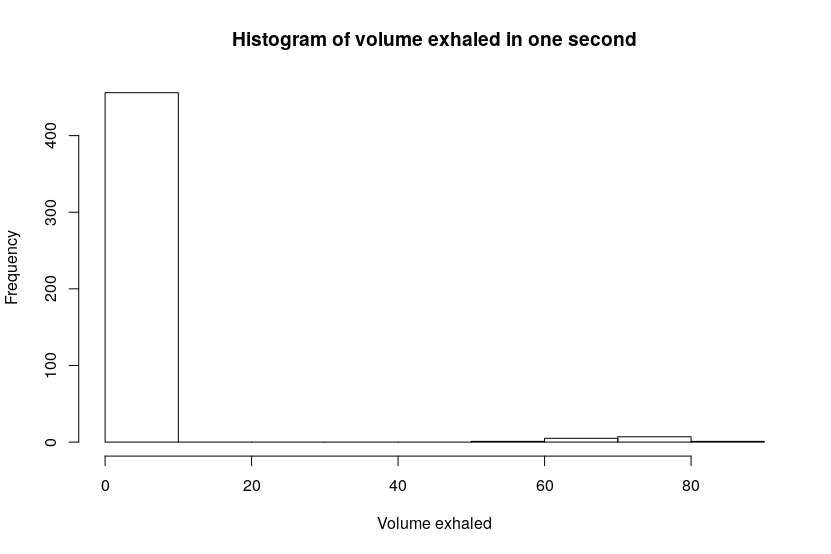
\includegraphics[width=10cm]{histFEV1}
\label{fig:histFEV1}
\caption{Show the ammount of people having each value}
\end{figure}
\subsubsection{Coding of non-continuous or non-ordered variables}
% \todo[inline]{El código que convierta nuestras variables categóricas en tiras
% de 0s y 1s}

\red{La mayoría de variables son binarias, y establecemos su tipo en "binary"}

\red{Las variables "PERFORMANCE" Y "SIZE" sí que tienen un orden, por lo tanto
las definimos como numeric (integer)}

\red{AGE se queda como está, numeric}

\red{Tanto PERFORMANCE como SIZE como AGE se normalizarán}

As most of the dataset variables are logical, we have coded them as logical in R. We have converted the variable ``DGN'' to many binary variables, each one saying wether the patient showed that diagnosis or not.

Originally, the variables ``PERFORMANCE'' and ``SIZE'' were categorical, but as they seem to have some kind of order, we have coded them as numeric. The ``PERFORMANCE'' can have values $1,2,3$ and the variable ``SIZE'' can have values $1,2,3,4$. Both of them are then normalized.

``AGE'' is also normalized in the range $[0, 100]$

\subsubsection{Possible elimination of irrelevant variables}

Some of the variables of our dataset are not well represented. In particular:

\begin{center}
\begin{tabular}{|c|c|}
  \hline
  \textbf{DGN} & There is just one patient with DGN = 1 and just 8 have DGN = 8 \\
  \hline
  \textbf{PAD} & Just 8 patients have PAD = True \\
  \hline
  \textbf{ASHTMA} & Just 2 patients have ASHTMA = True \\
  \hline
\end{tabular}
\end{center}

Hence the normal thing to do would be to eliminate those columns in our dataset,
since they do not provide good information. However, as we have very few instances
we can afford to try out keeping and removing them. We will run our models with
each of the 16 combinations of keeping DGN1, DGN8, PAD and ASHTMA and we will
see which one works better.

% \todo[inline]{Redactar bien esta parte, indicando que puesto que tenemos pocos
% datos, podemos permitirnos hacer varias ejecuciones, y que probaremos cada
% combinación de eliminar y no eliminar cada una de estas variables y veremos
% cual da mejores resultados con la cross-validation}

%
% \red{Algunas variables están muy poco representadas:}
% \red{Haremos los experimentos dos veces, uno con todos los datos originales,
% y otro quitando el atributo de MI, ASHTMA, DGN1 y DGN8, y entonces veremos cual
% da mejores resultados}
% \begin{itemize}
%   \item DGN: Solo un paciente tiene DGN1, y solo 2 tienen DGN8
%   \item Solo 2 pacientes tienen MI == True
%   \item Solo 8 pacientes tienen PAD == True
%   \item Solo 2 pacientes tienen ASHTMA == True
% \end{itemize}

\red{Mirar si podemos agrupar varios DGN que se parezcan (preguntar a alguien que sepa)}

\red{Haremos 2 datasets, uno que sea el original sin quitar nada, otro en el que
quitaremos cosas}

\red{Seguro que quitamos DGN1, DGN8, MI,  y ASTHMA}
\subsubsection{Creation of new useful variables (Feature extraction)}
\red{Entender cómo funciona MCA, y ver si podemos sacar una variable nueva}

\red{Quizá es interesante añadir la variable FEV/FEV1}
\subsubsection{Normalization of the variables}
We need to normalize only our numeric variables, which are the AGE, FVC and FEV1.
To normalize the age we will only consider cases between $0$ and $100$ years old.
For FVC and FEV1 the range will correspond to the maximum and minimum observed values with a margin of 10\%.

% For FVC and FEV1 the maximum will correspond to $1.1K_{FVC}$ and $1.1K_{FEV1}$,
% where $K_{FVC}$ is the maximum observed FVC and $K_{FEV1}$ is the maximum
% observed FEV1.


% \red{Sería posible hacer la edad más ajustada, entre el máximo y el mínimo}

% \red{Hablar sobre ese 1.2 (podría ser cualquier otro)}

% \red{Quizá se puede usar el mismo máximo para FVC y FEV1, que sería el que
% corresponde a FVC, pues el es mayor}

\red{Si finalmente añadimos el atributo FEV1/FVC, indicar que no hace falta
estandarizarlo puesto que ya lo está}

\red{Puesto que al final PERFORMANCE y SIZE las hemos puesto como numéricas, también las hemos normalizado. Explicarlo}

% \red{El margen solo será del 10\%}

% \red{Solo se pueden normalizar FVC, FEV1 y AGE. Miraremos cuales dan mejores
% resultados}
\subsubsection{Transformation of the variables}
Acording to \red{the paper we found} the accetable range for skewness in a numeric
variable is $(-2, +2)$. The skewness of our original variables AGE, FVC and FEV are:

\begin{center}
\begin{tabular}{| c | c |}
  \hline
  AGE & -0.1899413 \\
  FVC & 0.5417132 \\
  FEV1 & 5.597584 \\
  \hline
\end{tabular}
\end{center}

But we have to take into account that we've eliminated \red{22} patients, so the
new values are:

\todo[inline]{Poner los nuevos valores}

As the three variables are in the specified range, there is no need of
transforming them.

% \red{Skewness es la asimetría de los datos respecto a la media.}
% \red{Como la mayoría de nuestras variables son categóricas, no tiene mucho
% sentido medir el skewness, ni tampoco corregirlo}
% \red{Kurtosis igual que el skewness, no es necesario porque la mayoría con
% categóricas}
 % consultar si debemos ignorar este punto
% \todo[inline]{El código en r para corregir la asimetría (skewness) de los datos}
% \red{Es aceptable un skewness entre -2 y +2. AGE y FVC ya están en este rango, por
% lo tanto no hay que hacer nada con ellos. FEV1 sí que se sale, pero los datos que
% tiene son erroneos. Por lo tanto los transformatemos de alguna forma (eliminarlos
% o inferirlos) y miraremos el skewness de esos nuevos datos. (suponemos que entonces
% sí que estarán en ese rango, y por tanto no habrá que aplicar la transformación)}

\red{Referenciar (y leer un poco...) el paper}


%https://www.researchgate.net/publication/281345819_The_Research_Methods_Knowledge_Base


% \subsection{Feature extraction/selection}
\subsection{Clustering}
\red{hacer varios k-means con distintos valores de k (2,3,4,5,6) para ver si descubrimos algún cluster que nos permita crear una variable nueva}
\subsection{Visualization}
\red{Hacer MCA  }
